\documentclass[14pt]{beamer}
\title{OTHELLO}
\date{26-10-2021}
\author[Bvrith]{Richa cristina: 20WH1A0576: CSE \\P Meghana: 20WH1A12A8: IT\\K Sushmeetha: 20WH1A1258: IT\\G Alekhya: 20WH1A0432: ECE\\P Aruna: 20WH1A0237: EEE\\Bushra Mahaveen: 21WH5A0204: EEE}
\usefonttheme{serif}
\usepackage{bookman}
\usepackage{hyperref}
\usepackage[T1]{fontenc}
\usepackage{graphicx}
\usecolortheme{orchid}
\beamertemplateballitem

\begin{document}
    \begin{frame}
        \titlepage
          \begin{center}
	        Team 85
	      \end{center}
    \end{frame}
    \begin{frame}
	\frametitle{Introduction}
        \begin{itemize}
	    \item  Othello is a game played by two people on an 8 x 8 board.
		\vspace {0.2in}
               \begin{figure}
                   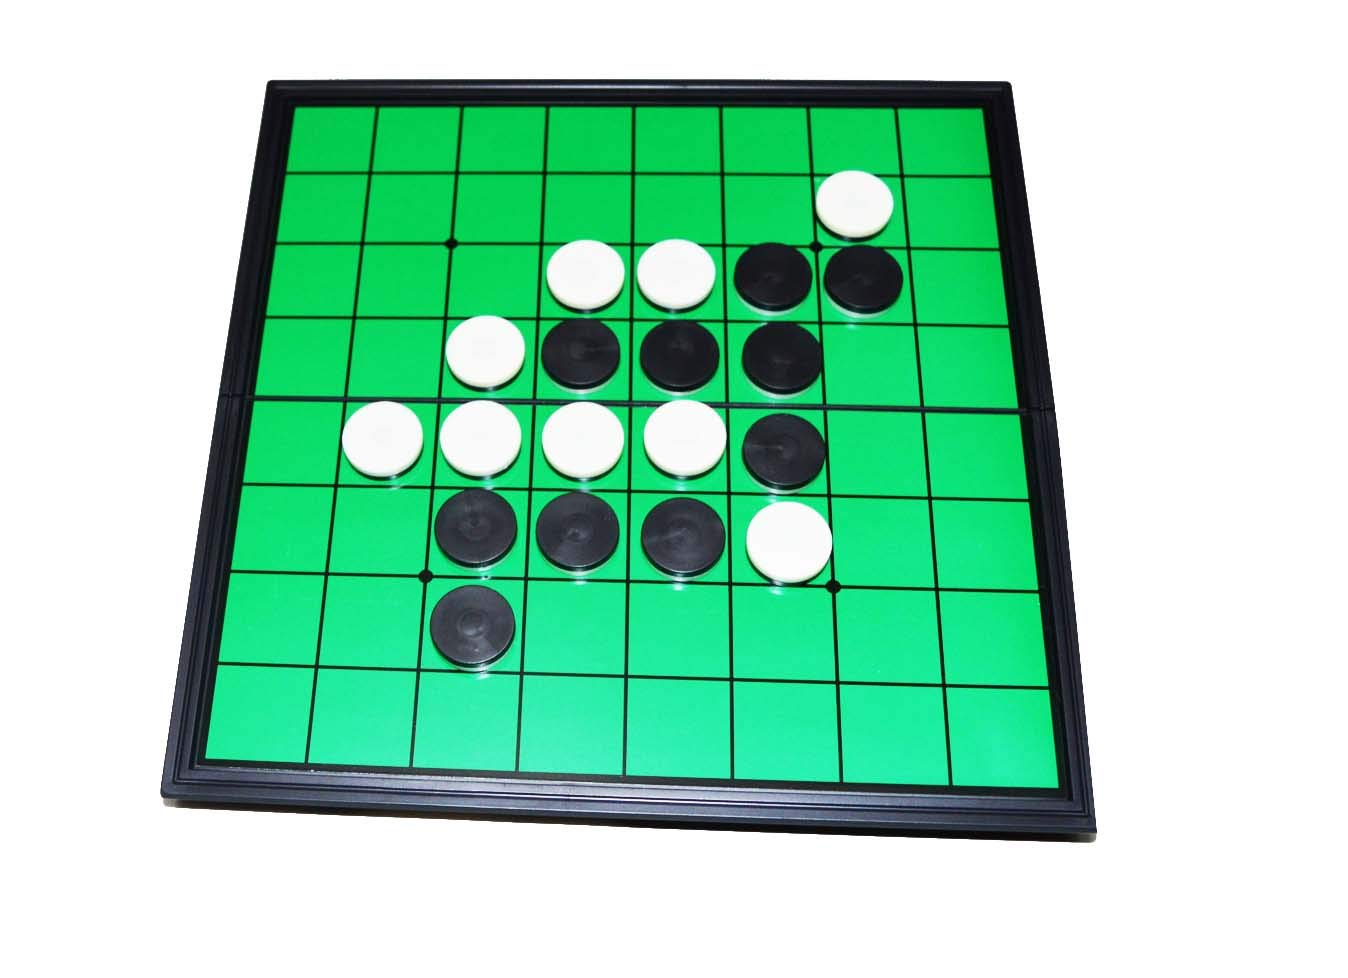
\includegraphics [width=7cm] {othellobg.jpg}
               \end{figure}
	\end{itemize}
    \end{frame}
    \begin{frame}
	\frametitle{Approach}
	\begin{itemize}
	    \item Creating 8 x 8 grid
           \item Taking input from the player
           \item Placing the coins according to the input
	\end{itemize}
    \end{frame}

    \begin{frame}
          \begin{center}
	          Demo of the project
	     \end{center}
     \end{frame}

 \begin{frame}
	\frametitle{Challenges}
        \begin{itemize}
	     \item Defining the legal moves
           \item Placing the coins on the board
     \end{itemize}
\end{frame}
    \begin{frame}
        \frametitle{Learnings}
	\begin{itemize}
	      \item LaTeX
            \item Gitlab
             \item Teamwork
	\end{itemize}
    \end{frame}

\begin{frame}
    \frametitle {Tech Stack}
     \begin{itemize}
         \item OS : Windows 10
          \item Language : Python 3.9
           \item MiKTeX
       \end{itemize}
\end{frame}
   
  \begin{frame}
      \frametitle{GIT}
         \begin{figure}
             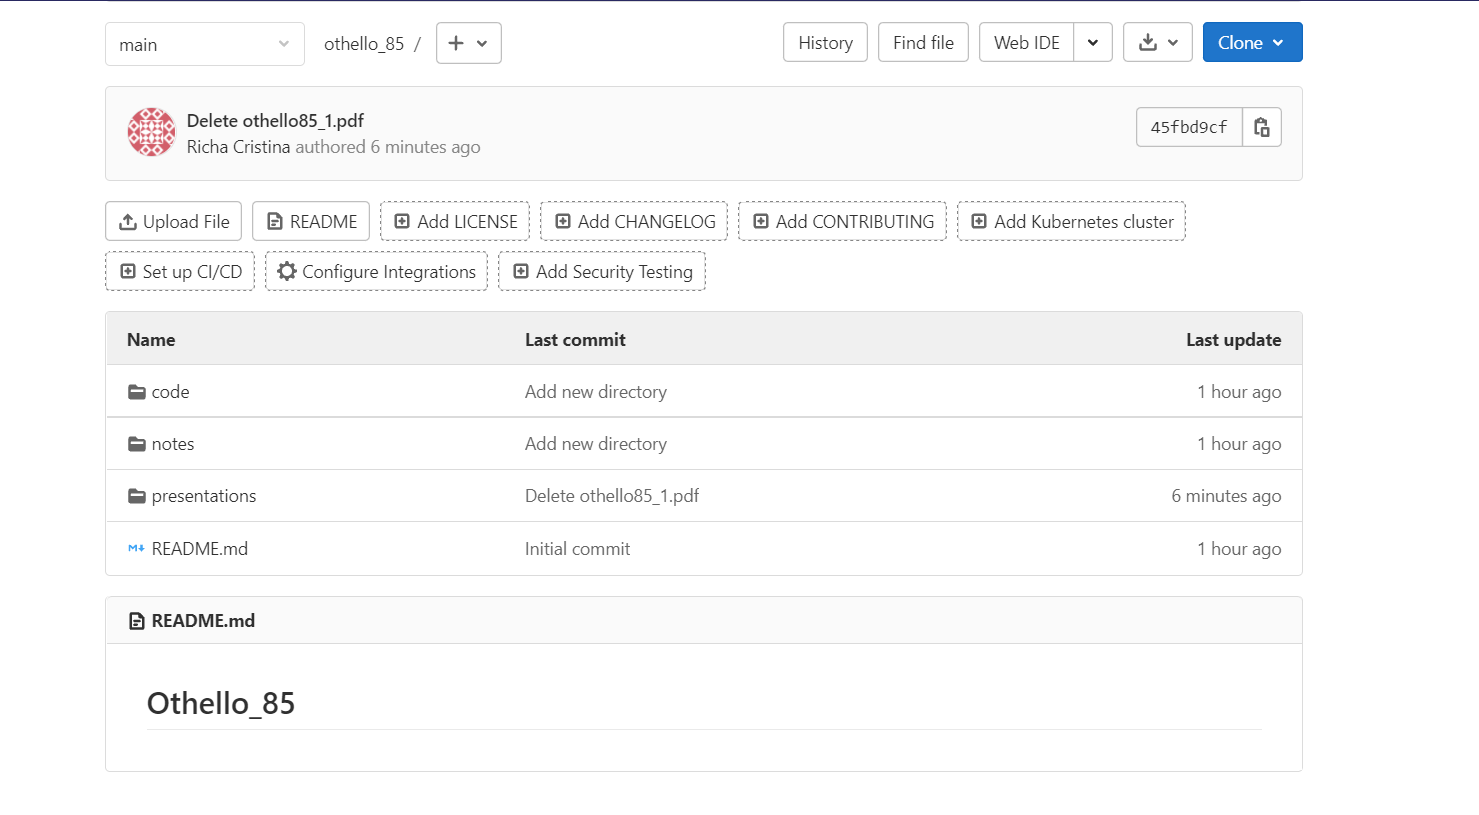
\includegraphics [width = 10cm] {repository.png}
         \end{figure}
      \end{frame}
 \begin{frame}
    \frametitle {Statistics}
      \begin {itemize}
        \item Number of lines of code - 110
         \item Number of functions - 9
        \end {itemize}
\end{frame}
    \begin{frame}
	\begin{center}
	     Thank you!!!
	\end{center}
    \end{frame}
\end{document}
